\chapter{Approfondimenti teorici}\label{chap:approfondimenti_teorici}

\section{Problema della separabilità non lineare nel percettrone}\label{sec:separabilita_non_lineare}
\textit{Questa parte è tratta dal capitolo \ref{chap:primi_modelli}, dove si parla del percettrone nella sezione \ref{sec:modelli_lineari}.}

\paragraph{Definizione (separabilità lineare).}
Sia $X=\{x^{(1)},\ldots,x^{(m)}\}\subset\mathbb{R}^{d}$ e sia $y\in\{0,1\}^{m}$ un insieme di etichette.
Diciamo che i due insiemi di punti $A=\{x^{(i)}:y^{(i)}=1\}$ e $B=\{x^{(i)}:y^{(i)}=0\}$ sono \emph{linearmente separabili} se esistono $w\in\mathbb{R}^{d}$ e $b\in\mathbb{R}$ tali che
\[
w^\top x \;>\; b \quad \forall x\in A,
\qquad
w^\top x \;<\; b \quad \forall x\in B.
\]
Equivalente: esiste un iperpiano $w^\top x=b$ la cui parte positiva contiene tutti i punti di $A$ e la parte negativa tutti i punti di $B$.

\paragraph{Quante funzioni booleane sono linearmente separabili?}
Per $m$ argomenti binari esistono $2^{2^{m}}$ funzioni booleane possibili; solo una parte è realizzabile con un singolo classificatore lineare.
Dati noti:
\[
\begin{array}{lcl}
m=2 &\Rightarrow& 14 \text{ su } 16 \text{ sono separabili linearmente},\\[2pt]
m=3 &\Rightarrow& 104 \text{ su } 256 \text{ sono separabili linearmente},\\[2pt]
m=4 &\Rightarrow& 1882 \text{ su } 65536 \text{ sono separabili linearmente}.
\end{array}
\]
Non esiste una formula chiusa semplice che dia, in funzione di $m$, quante funzioni sono linearmente separabili; tuttavia si osserva che, all’aumentare di $m$, la \emph{frazione} di funzioni separabili decresce rapidamente.

\paragraph{Dicotomie di un insieme di punti.}
Dato $X=\{x^{(1)},\ldots,x^{(m)}\}\subset\mathbb{R}^{d}$, le possibili etichettature (o \emph{dicotomie}) sono $2^{m}$:
\[
\mathcal{Y}=\{0,1\}^{m} .
\]
Solo una parte di queste dicotomie è realizzabile mediante una frontiera lineare. Con $d$ fissata, il numero di dicotomie realizzabili cresce in modo polinomiale in $m$ (ordine al piu $m^{d}$), mentre il totale cresce esponenzialmente ($2^{m}$); di conseguenza,
\[
\Pr\{\text{dicotomia separabile linearmente}\}\;\longrightarrow\;0
\quad\text{quando } m \gg d .
\]

\begin{figure}[htbp]
	\centering
	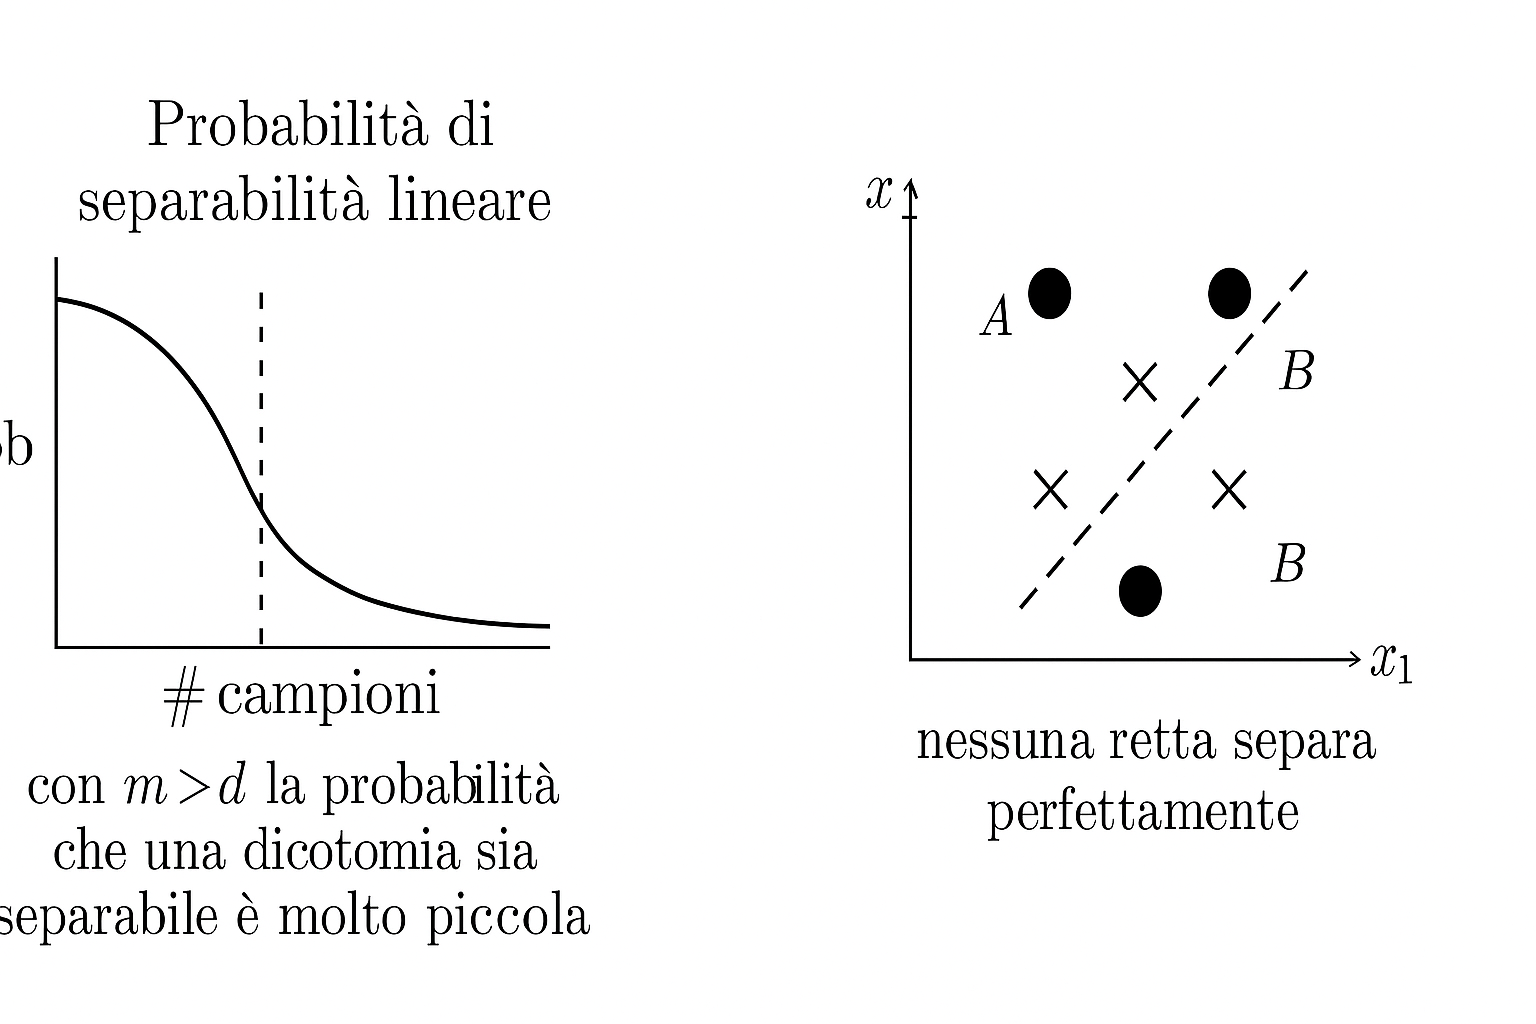
\includegraphics[width=0.7\linewidth]{images/non_linear_separation-probability.png}
	\caption{Separabilità non lineare. A sinistra: andamento qualitativo della probabilità che una dicotomia sia linearmente separabile al crescere del numero di campioni \(m\) (con dimensione \(d\) fissata); a destra: esempio in \(\mathbb{R}^2\) di punti non separabili con un singolo iperpiano.}
	\label{fig:nonlinear-separability}
\end{figure}

Intuitivamente: se il numero di campioni cresce molto a parità di dimensione $d$, è sempre meno probabile che una separazione perfetta con una sola retta/iperpiano esista.


\section{Generalizzazione funzione di costo del softmax}\label{sec:softmax_generalizzazione_logistica}
\textit{Questa parte è tratta dal capitolo \ref{chap:classificazione} nella sezione \ref{sec:proprieta_softmax}.}

Il modello softmax è una generalizzazione della regressione logistica multiclasse, si può infatti dimostrare che la funzione di costo del softmax riduce a quella della regressione logistica binaria per $K=2$ classi.
Ricordiamo che la funzione di costo del softmax è:
\[
J(\vartheta)
= -\frac{1}{m}\sum_{i=1}^{m}\sum_{c=0}^{K-1}
\mathbf{1}\{y^{(i)}=c\}\,\log\!\big(h_{\vartheta}^{(c)}(x^{(i)})\big)
+\frac{\lambda}{2}\sum_{c=0}^{K-1}\sum_{j=1}^{n}(\vartheta_j^{(c)})^2,
\]

É facile vedere che, per $K=2$ (senza regolarizzazione) vale:
\begin{align*}
J(\vartheta)
&= -\frac{1}{m}\sum_{i=1}^{m}\sum_{c=0}^{1}
\mathbf{1}\{y^{(i)}=c\}\,\log\!\big(h_{\vartheta}^{(c)}(x^{(i)})\big)\\
&= -\frac{1}{m}\sum_{i=1}^{m}
\Big[\mathbf{1}\{y^{(i)}=0\}\log h_{\vartheta}^{(0)}(x^{(i)})
     +\mathbf{1}\{y^{(i)}=1\}\log h_{\vartheta}^{(1)}(x^{(i)})\Big]\\
&= -\frac{1}{m}\sum_{i=1}^{m}
\Big[(1-y^{(i)})\log h_{\vartheta}^{(0)}(x^{(i)})
     +y^{(i)}\log h_{\vartheta}^{(1)}(x^{(i)})\Big]\\
&= -\frac{1}{m}\sum_{i=1}^{m}
\Big[(1-y^{(i)})\log\!\big(1-h_{\vartheta}^{(1)}(x^{(i)})\big)
     +y^{(i)}\log h_{\vartheta}^{(1)}(x^{(i)})\Big],
\end{align*}

dove si è usata la normalizzazione della softmax $h_{\vartheta}^{(0)}(x)+h_{\vartheta}^{(1)}(x)=1$.
Questa è esattamente la loss della regressione logistica binaria: dunque la regressione logistica è un caso particolare della softmax.

Si può ulteriormente dimostrare che il softmax è una generalizzazione della regressione logistica multiclasse usando una sua proprietà principale: l'\emph{overparametrizzazione}. Per $K=2$:
\[
h_{\vartheta}(x)=
\begin{bmatrix}
\dfrac{e^{\vartheta^{(0)\!\top}x}}{e^{\vartheta^{(0)\!\top}x}+e^{\vartheta^{(1)\!\top}x}}\\[6pt]
\dfrac{e^{\vartheta^{(1)\!\top}x}}{e^{\vartheta^{(0)\!\top}x}+e^{\vartheta^{(1)\!\top}x}}
\end{bmatrix}
=
\begin{bmatrix}
\dfrac{e^{(\vartheta^{(0)}-\vartheta^{(1)})^\top x}}{e^{(\vartheta^{(0)}-\vartheta^{(1)})^\top x}+e^{\mathbf 0^\top x}}\\[6pt]
\dfrac{e^{(\vartheta^{(1)}-\vartheta^{(1)})^\top x}}{e^{(\vartheta^{(0)}-\vartheta^{(1)})^\top x}+e^{\mathbf 0^\top x}}
\end{bmatrix}
=
\begin{bmatrix}
\dfrac{e^{\Delta^\top x}}{1+e^{\Delta^\top x}}\\[6pt]
\dfrac{1}{1+e^{\Delta^\top x}}
\end{bmatrix},
\qquad \Delta=\vartheta^{(0)}-\vartheta^{(1)}.
\]
Ponendo \(\mathbf w=\vartheta^{(1)}-\vartheta^{(0)}=-\Delta\) e
\(\sigma(z)=\dfrac{1}{1+e^{-z}}\) si ottiene
\[
h_{\vartheta}(x)=
\begin{bmatrix}
1-\sigma(\mathbf w^\top x)\\[4pt]
\sigma(\mathbf w^\top x)
\end{bmatrix}.
\]

\noindent
Quindi, per $K=2$, il softmax riduce alla regressione logistica binaria.
